\documentclass[
    a4paper,
    % bibliography=totoc,
    12pt,
    parskip=half,
]{scrarticle}

\usepackage[T1]{fontenc}
\usepackage{mlmodern}
\usepackage[english]{babel}
\usepackage{blindtext}

\usepackage{graphicx} % Required for inserting images
\usepackage{enumitem}
\usepackage{amsmath}
\usepackage[left=2cm,right=2cm]{geometry}
% \usepackage[backend=biber, style=ieee, maxbibnames=6, minbibnames=1, maxcitenames=3, mincitenames=1]{biblatex}
\usepackage{hyperref}
% \hypersetup{
%     colorlinks=true,
%     citecolor=blue,
% }
\usepackage{subcaption}

% Don't show subsubsection in TOC
\setcounter{tocdepth}{2}

\graphicspath{{images}}

\title{Assignment 2 Report}
\author{Grübling Alexander (12122371) \\ Preissegger Leo (12122526) \\  Seczer Tobias (12119044) \\ Shanto Md Aminul Islam (12310834) }
\date{\today}

\pagenumbering{gobble}
\begin{document}

\thispagestyle{empty}
\begin{titlepage}
    \makeatletter
    \centering
    {\LARGE \bfseries \sffamily \@title \par}
    \vspace{3\baselineskip}
    {\large \bfseries \sffamily Group 10 \par}
    {\large \@author \par}
    {\large \@date \par}
    \vspace{2\baselineskip}
    \vfill{}
    {\large
    183.630 \\
    Medical Image Processing UE \\
    Semester: S2025 \par}
    \makeatother
\end{titlepage}

\pagenumbering{arabic}

\begin{enumerate}
    \item Data Exploration
    \begin{enumerate}[label=\theenumi.\arabic*.]
        \item Simple \texttt{plt.imshow} together with \texttt{plt.scatter}
        \item Same as 1.1., but the aligned landmarks are centered around \((0, 0)\).
        \item The scale factor can just be applied to the normal data shape, as it's uniform for all axes.
        We then need to add the rotation matrix, which is very simple in 2D. In order to apply the rotation matrix,
        we also need to reshape from \([x_1, \ldots , x_N, y_1, \ldots, y_N]\) to \([[x_1, \ldots, x_N], [y_1, \ldots, y_N]]\), then apply
        the rotation matrix. Lastly, we just need to add the translation to the result and reshape it back to the original shape.
        \item We used the PCA module of sklearn.
        I tested the methods with angles and translations of which I knew how the output should look like and it was ok,
        so the final output with our calculated transformations should also be correct.
    \end{enumerate}

    \item Feature Extraction and Edge Detection via Convolutions
    \begin{enumerate}[label=\theenumi.\arabic*.]
        \item Edge Detection via Convolutions
        \begin{enumerate}[label=\alph*)]
            \item Here the two Prewitt kernels are defined as numpy arrays in the variable \texttt{PREWITT\_X} and \texttt{PREWITT\_Y}.
            The values of the kernels are taken from the assignment sheet.
            \item The convolution is done by first padding the image with one zero on each side to avoid problems with the borders.
            Then we use a nested for loop to iterate over the image and apply the convolution by extracting  a \(3 \times 3\) patch of the image and multiplying it with the kernel.
            \item Now three images are randomly sampled from the dataset using \\ \texttt{np.random.choice(len(images), size=3, replace=False)}.
            After the images ares sampled, the convolution is applied to each of them using the function \texttt{conv2d(...)} defined in 2.1.b.
            Finally, the convolved images are plotted.
        \end{enumerate}
        \item Image Feature Computation:
        The implementation of this task was pretty straight forward. As we already get a grayscaled image, we can just flatten the array to receive the grayscaled values. To get the gradients, we rely on the Prewitt kernels created before as well as the convolution function. The magnitude of the gradients are then given by the absolute values of the result. With \texttt{np.meshgrid} we then create a grid of the original image's shape. Lastly, we stack all of the results vertically to get the feature matrix as requested by the task description.
    \end{enumerate}

    \item Classification and Feature Selection
    \begin{enumerate}[label=\theenumi.\arabic*.]
        \item Data preparation
        \begin{enumerate}[label=\alph*)]
            \item Splitting the image dataset of 50 images with its corresponding masks where 30 images \texttt{(I\_train)}  and \texttt{masks (y\_train)} use for training. The rest of them are used for testing the Random Forest algorithm. The test images and their masks denote \texttt{I\_test} and \texttt{y\_test}, respectively.
        \end{enumerate}
        \item Random Forest (RF)
        \begin{enumerate}[label=\alph*)]
            \item \texttt{RandomForestClassifier} uses from \texttt{sklearn} module. The parameters are \texttt{n\_estimators}, \texttt{max\_features}, \texttt{class\_weight}, \texttt{n\_jobs}, \texttt{oob\_score}, and \texttt{random\_state}. n\_estimators are the number of trees, in the \texttt{Random Forest} algorithm, 100 trees are used for better performance and accuracy.
            To reduce the overfitting and ensuring the diversity of the trees, max\_features parameters are set to \texttt{"sqrt"}. To automatically adjust the weights of the target variable, \texttt{class\_weight} set to "balanced" and utilizing multiple CPU cores of local machine, n\_jobs set to -1. To estimate the generalization accuracy - Out\-of\-bag samples are used, hence \texttt{oob\_score} set to "True". Better oob\_score means the model will perform better with the unseen data. lastly, random\_state ensures the reproducibility of results. \texttt{clf.fit(X\_train\_flat, y\_train\_flat)} trains over the samples and features. 
            \item The Random Forest Algorithm trains on 36,598 pixels with 7 features. Since the out\-of\-bag score calculates validation accuracy of unused samples during training - therefore, 0.939 score means the model will perform well with the random data.
            \item The Random Forest Classifier has Dice score 0.23, precision 0.13, and Recall of 0.79. The dice score suggested that the segmentation is very weak. because of the severe class imbalance what could be seen from confusion matrix and shallow feature set, makes it hard for the trees to learn.  
        \end{enumerate}
        
        \item U-Net
        \begin{enumerate}[label=\alph*)]
            \item We can see that the loss function for the unaugmented U-Net looks quite bad.
            The validation and training loss decrease until around epoch 40.
            Afterwards, only the training loss decreases while the validation loss increases, which means the model is overfitting to the training data and cannot generalise well.
            For the augmented U-Net, both the training and validation loss steadily decrease until the end of the training.
            This is because the data augmentation introduces random transforms, such as flipping the image, changing brightness/contrast, or elastic transform, which means that the U-Net will not overfit like before.\\
            \begin{minipage}{\linewidth}
                \centering
                \begin{minipage}{0.5\linewidth}
                    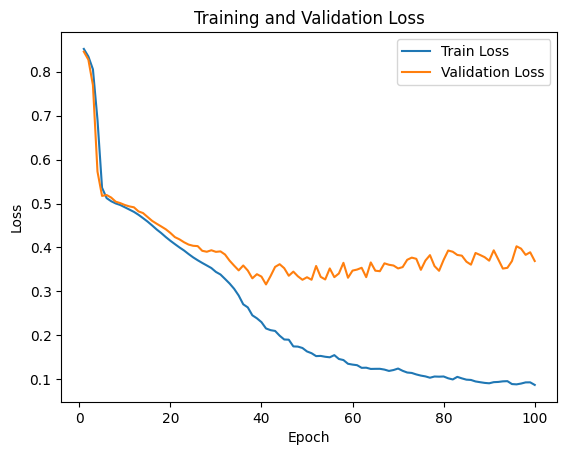
\includegraphics[width=\linewidth]{unet_loss}
                    \captionof{figure}{Unaugmented U-Net Loss}
                    \label{fig:unet_loss}
                \end{minipage}%
                \begin{minipage}{0.5\linewidth}
                    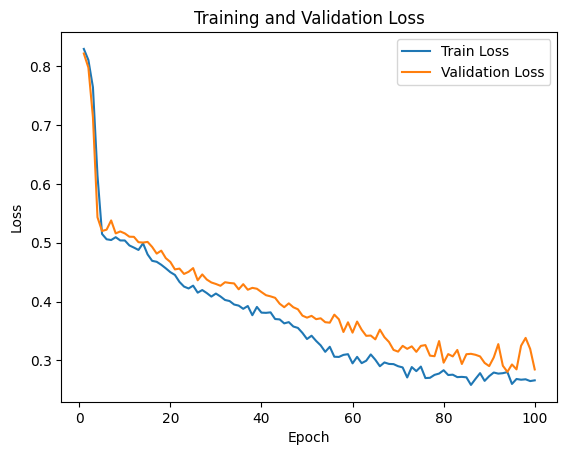
\includegraphics[width=\linewidth]{unet_augmented_loss}
                    \captionof{figure}{Augmented U-Net Loss}
                    \label{fig:unet_augmented_loss}
                \end{minipage}
            \end{minipage}
            \item It looks like channel 2 learned to detect edges of the image.
            Channel 0 and 7 look quite similar, like a greyscale version of the input image, while channel 1 and 3 look pretty much just like the input.
            This could indicate that these channels are used to capture general information of the input image.
            Channel 4, 5, and 6 all look very dark and almost inverted from the input image, which could indicate that they are used to learn something from the background brightness.
            Especially in channel 5 we can see the middle top part of the middle bone, so it might learn to extract the shape of the top part of the middle bone. \\
            \begin{minipage}{\linewidth}
                \centering
                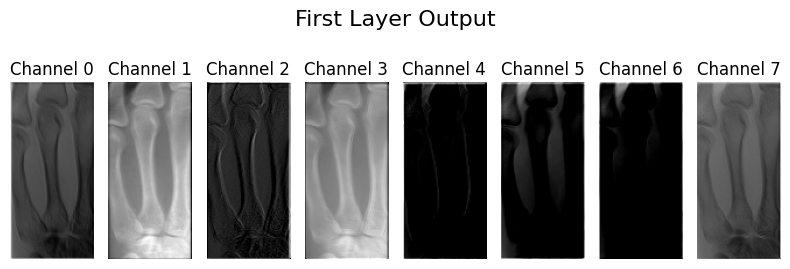
\includegraphics[width=\linewidth]{unet_layers}
                \captionof{figure}{U-Net first layer outputs}
                \label{fig:unet_layers}
            \end{minipage}
            \item Now we use the U-Net to predict the segmentation masks for the test images.
            To do so, we first need to create a dataset and a dataloader for the test images, because the U-Net expects the images to be in a specific shape, that the dataloader automatically produces.
            In order to plot the predicted masks, we need to convert them back to numpy arrays and use the \texttt{plot\_prediction\_triplets(...)} function with the input images, the predicted masks, and the ground truth masks.
            \item For the random forest, we achieve a Dice Score of 0.231, a Precision of 0.135, and a Recall of 0.794.
            The U-Net without augmentation achieves a Dice Score of 0.11, a Precision of 0.059, and a Recall of 0.99.
            When the U-Net is trained with augmentation, it achieves a Dice Score of 0.028, a Precision of 0.014, and a Recall of 1.0.
            \\
            The Random Forest preforms significantly better than both U-Net models.
            The main problem with the U-Net is probably the small dataset size, which is not enough to train a deep learning model like U-Net.
            Especially for the not augmented U-Net, we see overfitting, as the models loss stays constant or even goes up, starting with epoch 40.
            However, the Train Loss is still decreasing.
            The augmentation does also not help in this case.
            \\
            However, the results that are plotted in Task 3.3c) show that the U-Net is able to learn some features of the segmentation masks, as it is able to predict some of the masks correctly.
            Regarding that, I do not really understand why the recall is that high.
        \end{enumerate}
        \item Shape Particle Filters
        \begin{enumerate}[label=\alph*)]
            \item First we need to define a cost function, based on a given shape model as well as a classification. The function we have chosen is rather straightforward, which may explain the arguably poor results obtained and plotted in Task 3.4b). We compute the euclidean distance of each classified segmentation to the nearest pixel identified by the shape model. We then return the average of these distances as cost.\\
            In \texttt{fit\_shape\_model}, we then aim at optimizing based on this cost function. To do that, all we really have to do is define the bounds for that optimization process, and the rest will be done for us by the \texttt{optimize} function that was supplied to us.\\
            For parameter \texttt{b}, we allow up to three standard deviations of variance for each component. \texttt{scale} we allow in the bounds of 0.5 to 2 as a means of resizing of the shape.  For rotation, we allow in between -Pi and Pi Radians. Then for translations we allow half the image up or downwards in both directions.
            \item The green lines are the ground-truth contour and the red dotted line is the predicted mask which is derivated by the Random-Forest algorithm. The pipeline performs well where the cortices are thick and high-contrast as the forest heavily depends on the raw density. But the model struggles in the thin cortext and bone overlaps, noisy background is another issue.
            Bright soft-tissue  and overlapping bones also created false-positive pixels which creates misplaced or rotated masks. Class balances and feature engineering will improve the random forest classifier. Iterative shape fitting can also improve the precision and dice score simultaneously. 
        \end{enumerate}
    \end{enumerate}
\end{enumerate}

\end{document}